\documentclass[tikz,border=10pt]{standalone}
\usepackage{tikz}
\usetikzlibrary{positioning, fit, arrows.meta, backgrounds, calc, shadows, shapes.geometric, shapes.misc, shapes.symbols}

\begin{document}
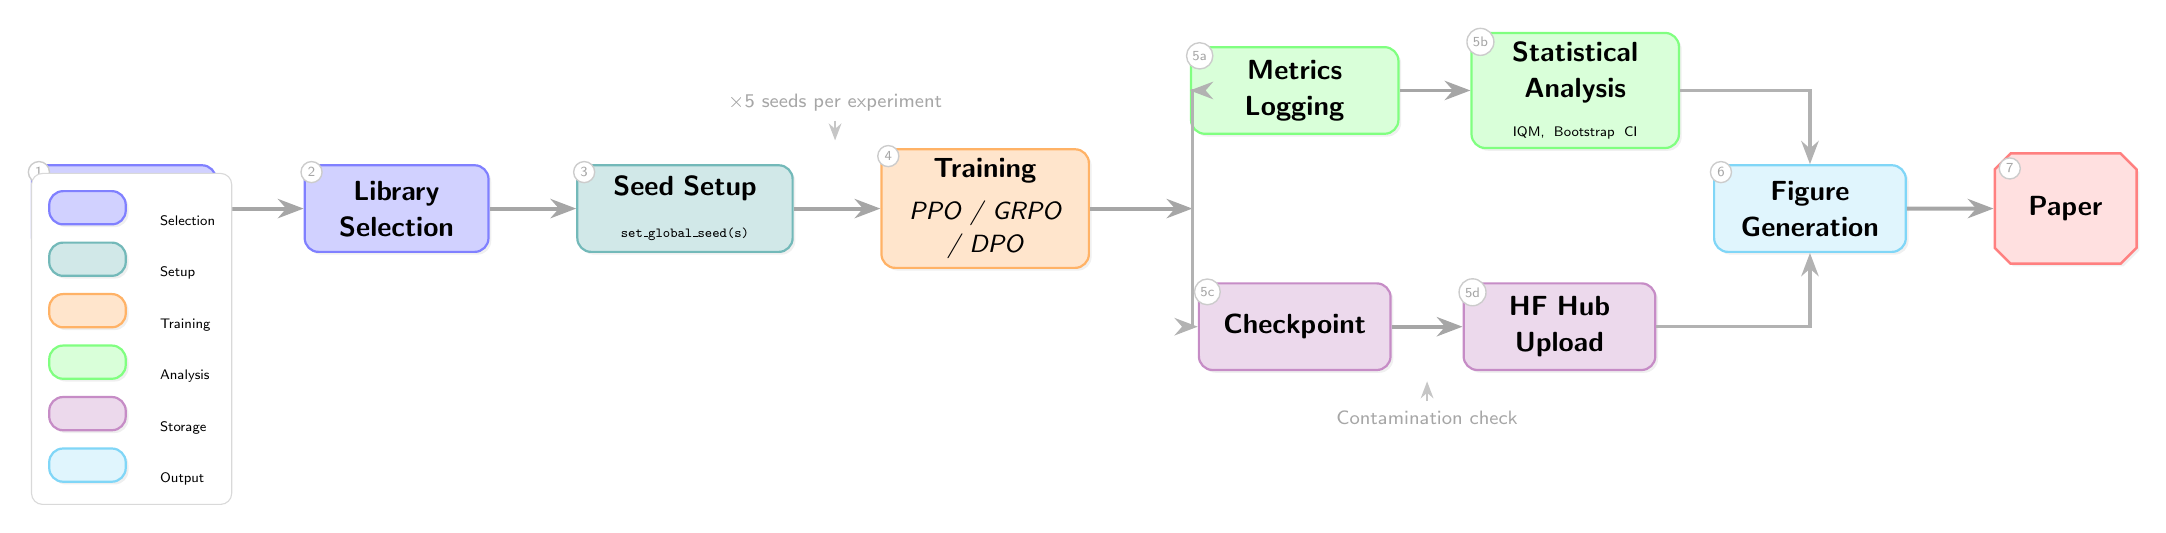
\begin{tikzpicture}[
  font=\sffamily,
  %% Main flow node — rounded rectangle
  flownode/.style={
    draw, rounded corners=5pt, align=center,
    minimum height=1.1cm, minimum width=2.3cm,
    line width=0.8pt,
    drop shadow={shadow xshift=1pt, shadow yshift=-1pt, opacity=0.12}
  },
  %% Specific color variants
  selectnode/.style={flownode, fill=blue!18, draw=blue!50, text width=2.1cm},
  setupnode/.style={flownode, fill=teal!18, draw=teal!55, text width=2.5cm},
  trainnode/.style={flownode, fill=orange!20, draw=orange!60,
                    minimum height=1.4cm, text width=2.4cm},
  metricsnode/.style={flownode, fill=green!15, draw=green!50, text width=2.4cm},
  checknode/.style={flownode, fill=violet!15, draw=violet!45, text width=2.2cm},
  fignode/.style={flownode, fill=cyan!12, draw=cyan!50, text width=2.2cm},
  %% Document shape for "Paper"
  papershape/.style={
    draw, chamfered rectangle,
    align=center, minimum height=1.4cm, minimum width=1.8cm,
    fill=red!12, draw=red!50, line width=0.9pt,
    drop shadow={shadow xshift=1pt, shadow yshift=-1pt, opacity=0.12}
  },
  %% Arrow style
  mainarrow/.style={-Stealth, line width=1.4pt, color=gray!70},
  forkarrow/.style={-Stealth, line width=1.2pt, color=gray!60},
  %% Annotation label
  annot/.style={font=\sffamily\scriptsize, text=gray!70, align=center},
]

%% ──────────────────────────────────────────────────────────
%% MAIN FLOW — left to right, y = 0
%% ──────────────────────────────────────────────────────────

%% 1. Task Selection
\node[selectnode] (tasksel) at (0,0)
  {\textbf{Task}\\[1pt]\textbf{Selection}};

%% 2. Library Selection
\node[selectnode] (libsel) [right=1.1cm of tasksel]
  {\textbf{Library}\\[1pt]\textbf{Selection}};

%% 3. Seed Setup
\node[setupnode] (seed) [right=1.1cm of libsel]
  {\textbf{Seed Setup}\\[3pt]{\tiny\ttfamily set\_global\_seed(s)}};

%% 4. Training
\node[trainnode] (train) [right=1.1cm of seed]
  {\textbf{Training}\\[3pt]{\small\itshape PPO / GRPO / DPO}};

%% Fork point (invisible)
\coordinate (fork) at ([xshift=1.3cm]train.east);

%% Upper fork: Metrics Logging → Statistical Analysis
\node[metricsnode] (metlog) at ([xshift=2.6cm, yshift=1.5cm]train.east)
  {\textbf{Metrics}\\[1pt]\textbf{Logging}};

\node[metricsnode] (statana) [right=0.9cm of metlog]
  {\textbf{Statistical}\\[1pt]\textbf{Analysis}\\[2pt]{\tiny IQM, Bootstrap CI}};

%% Lower fork: Checkpoint → HF Hub Upload
\node[checknode] (ckpt) at ([xshift=2.6cm, yshift=-1.5cm]train.east)
  {\textbf{Checkpoint}};

\node[checknode] (hfup) [right=0.9cm of ckpt]
  {\textbf{HF Hub}\\[1pt]\textbf{Upload}};

%% Merge point (invisible) — aligns with figure node x
\coordinate (merge) at ([xshift=1.1cm]$(statana.east)!0.5!(hfup.east)$);

%% 6. Figure Generation
\node[fignode] (figgen) at ([xshift=1.8cm]$(statana.east)!0.5!(hfup.east)$)
  {\textbf{Figure}\\[1pt]\textbf{Generation}};

%% 7. Paper
\node[papershape] (paper) [right=1.1cm of figgen]
  {\textbf{Paper}};

%% ──────────────────────────────────────────────────────────
%% ARROWS
%% ──────────────────────────────────────────────────────────

%% Main straight flow
\draw[mainarrow] (tasksel) -- (libsel);
\draw[mainarrow] (libsel)  -- (seed);
\draw[mainarrow] (seed)    -- (train);

%% Train → fork point
\draw[mainarrow] (train.east) -- (fork);

%% Fork → upper path
\draw[forkarrow] (fork) |-  (metlog.west);

%% Fork → lower path
\draw[forkarrow] (fork) |- (ckpt.west);

%% Upper path: metlog → statana
\draw[mainarrow] (metlog) -- (statana);

%% Lower path: ckpt → hfup
\draw[mainarrow] (ckpt) -- (hfup);

%% Merge into figgen
\draw[forkarrow] (statana.east) -| (figgen.north);
\draw[forkarrow] (hfup.east)    -| (figgen.south);

%% figgen → paper
\draw[mainarrow] (figgen) -- (paper);

%% ──────────────────────────────────────────────────────────
%% ANNOTATIONS
%% ──────────────────────────────────────────────────────────

%% Above steps 3-4: ×5 seeds
\node[annot, above=0.45cm of $(seed.north)!0.5!(train.north)$]
  (seedannot) {\texttimes5 seeds per experiment};

%% Arrow pointing down to seed/train
\draw[-Stealth, gray!45, line width=0.7pt]
  (seedannot.south) -- ++(0,-0.25);

%% Below steps 5-6 upper path: contamination check (between fork paths)
\node[annot, below=0.38cm of $(ckpt.south)!0.5!(hfup.south)$]
  (contam) {Contamination check};

\draw[-Stealth, gray!45, line width=0.7pt]
  (contam.north) -- ++(0,0.25);

%% ──────────────────────────────────────────────────────────
%% BACKGROUND: subtle step-numbering circles
%% ──────────────────────────────────────────────────────────
\foreach \nd/\num in {tasksel/1, libsel/2, seed/3, train/4,
                      metlog/5a, statana/5b, ckpt/5c, hfup/5d,
                      figgen/6, paper/7}{
  \node[
    circle, fill=white, draw=gray!40, line width=0.5pt,
    inner sep=1.2pt, font=\sffamily\tiny, text=gray!70,
    anchor=north west
  ] at (\nd.north west) {\num};
}

%% ──────────────────────────────────────────────────────────
%% LEGEND BOX (bottom-left)
%% ──────────────────────────────────────────────────────────
\node[
  draw=gray!30, rounded corners=4pt, fill=white,
  inner sep=6pt, font=\sffamily\tiny,
  anchor=south west
] at ([xshift=0.0cm, yshift=-3.2cm]tasksel.south west) {
  \begin{tabular}{@{}ll@{}}
    \tikz\node[selectnode, minimum height=0.35cm, minimum width=0.55cm,
               text width=0.55cm, font=\sffamily\tiny]{}; & Selection \\[4pt]
    \tikz\node[setupnode,  minimum height=0.35cm, minimum width=0.55cm,
               text width=0.55cm, font=\sffamily\tiny]{}; & Setup \\[4pt]
    \tikz\node[trainnode,  minimum height=0.35cm, minimum width=0.55cm,
               text width=0.55cm, font=\sffamily\tiny]{}; & Training \\[4pt]
    \tikz\node[metricsnode,minimum height=0.35cm, minimum width=0.55cm,
               text width=0.55cm, font=\sffamily\tiny]{}; & Analysis \\[4pt]
    \tikz\node[checknode,  minimum height=0.35cm, minimum width=0.55cm,
               text width=0.55cm, font=\sffamily\tiny]{}; & Storage \\[4pt]
    \tikz\node[fignode,    minimum height=0.35cm, minimum width=0.55cm,
               text width=0.55cm, font=\sffamily\tiny]{}; & Output
  \end{tabular}
};

\end{tikzpicture}
\end{document}
